\documentclass[12pt]{exam}
\usepackage{amssymb,amsmath,amsfonts,mathtools} % useful math fonts and symbols
\usepackage{hyperref}
\usepackage{multicol, multirow}
\usepackage[inner=1.0in, outer=1.0in, top=1.0in, bottom=1.0in]{geometry}

\pagestyle{headandfoot}
\lhead{EC327}
\chead{Activity 4 - Penalty Kick Shootout}
\rhead{\today}
\runningheadrule 

\hypersetup{
    colorlinks=true,
    linkcolor=blue,
    filecolor=magenta,      
    urlcolor=cyan,
}

\title{Activity 4 - Penalty Kick Shootout}
\date{\today}

\begin{document}

\section*{Dixit Skeath and Riley, Chapter 8, question S6:}

Looking at Tudor and Fordor again, 
assume that the old, established company Tudor is risk averse,
whereas the would-be entrant Fordor
(which is planning to finance its project through venture capital)
is risk neutral. 
That is, Tudor’s utility is always the square root of its total profit
over both periods.
Fordor’s utility is simply the amount of its profit —if any—
during the second period. 
Assume that Tudor’s low per-unit cost is 5, as in Section 6.A.

\begin{enumerate}
  \item  Redraw the extensive-form game shown in Figure 8.7, 
  giving the proper payoffs for a risk-averse Tudor. 
  \begin{figure}[!h]
    \centering 
    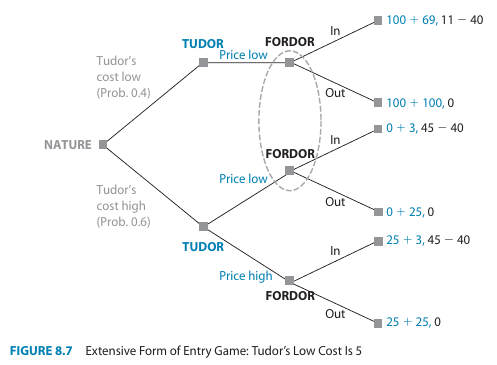
\includegraphics[width=.6\textwidth]{Fig8.8.png}
  \end{figure}
  \item Let the probability that Tudor is low cost, z, be 0.4. 
  Will the equilibrium be separating, pooling, or semiseparating? 
  (Hint: Use a table equivalent to Figure 8.8.) 
  \begin{table}[!h]
    \centering
    \begin{tabular}{cc|c|c|}
      & \multicolumn{1}{c}{} & \multicolumn{2}{c}{\textbf{Fordor}}\\
      & \multicolumn{1}{c}{} & \multicolumn{1}{c}{Regardless (II)}  & \multicolumn{1}{c}{Conditional (OI)} \\\cline{3-4}
      \multirow{2}*{\textbf{Tudor}}  & Bluff (LL) & &  \\[10ex] \cline{3-4}
      & Honest (LH) &  &  \\[10ex] \cline{3-4}
    \end{tabular}
  \end{table}
  \item Repeat part (2) with z = 0.1.
\end{enumerate}

\end{document}
